\input{configuration}

\title{Lecture 28 --- Data Warehousing \& Mining }

\author{Jeff Zarnett \\ \small \texttt{jzarnett@uwaterloo.ca}}
\institute{Department of Electrical and Computer Engineering \\
  University of Waterloo}
\date{\today}


\begin{document}

\begin{frame}
  \titlepage

 \end{frame}
 
 
\begin{frame}
\frametitle{Data Warehousing and Mining}

Think about a company like Amazon (let's restrict ourselves for the moment to their online store business). 

They have accumulated a huge amount of data about the purchases made. 

There needs to be a way to store this very large volume of data. That is what data \alert{warehousing} is about. 
 \end{frame}
 
 
\begin{frame}
\frametitle{Data Warehousing and Mining}


The purchase history of Amazon users between the years 2010 and 2015 is perhaps not needed on a regular basis, but it is saved and stored. 

\begin{center}
	
\includegraphics[width=0.75\textwidth]{images/museum.jpg}
\end{center}

But why? Because it can be \alert{mined}: it provides insights.

\end{frame}

\begin{frame}
\frametitle{Data Mining}

\alert{Data mining} is about extracting information from a large volume of stored data.  

The more data we have, the better predictions we can make. 

Amazon may know that 60\% of the time, someone who buys product $X$ will soon buy product $Y$.

They can suggest $Y$ to you on the page when you have added $X$ to your cart.


\end{frame}


\begin{frame}
\frametitle{This Got Creepy}

Now you might think that data mining is just helpful.

Amazon is guessing about products I want and if they guess right, they are helping me! 

Maybe? 

But the truth is, this sort of data mining can be downright... creepy.

\end{frame}

\begin{frame}
\frametitle{How Did It Know?}

Consider this story by Charles Duhigg, in the New York Times about Target...

\begin{center}
	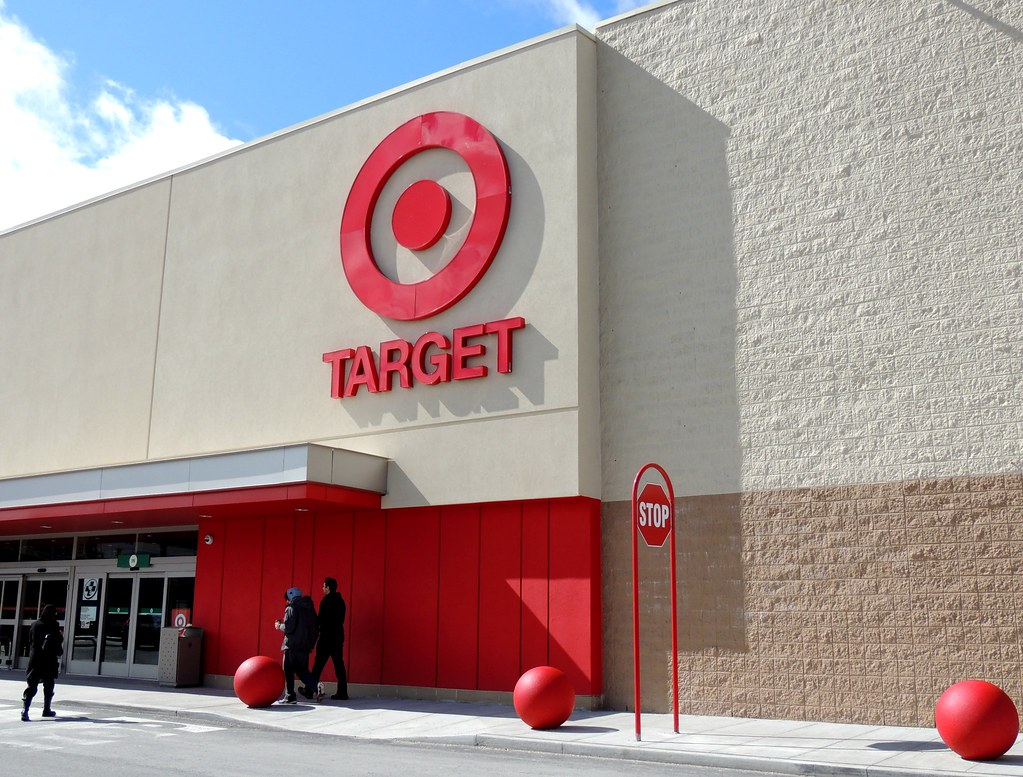
\includegraphics[width=0.6\textwidth]{images/target.jpg}
\end{center}

Used its data to make predictions about whether a woman is expecting a child...

\end{frame}

\begin{frame}
\frametitle{Data Warehousing}

Data warehousing is used to prepare large amounts of data for mining.

The purpose of the mining is to be used in a \alert{decision support system}. 

\begin{center}
	
\includegraphics[width=0.35\textwidth]{images/draw25.jpg}
\end{center}

\end{frame}

\begin{frame}
\frametitle{Decision Support System}

These are used to (for example):

\begin{itemize}
 \item Guess super personal information about shoppers
 \item Tell store managers what products they should stock in what month
 \item Tell factory managers what products they should manufacture
 \item Tell admissions officers what applicants should be admitted to a university
\end{itemize}

\end{frame}


\begin{frame}
\frametitle{Warehousing}

It is virtually a certainty that in any large organization, the data will be spread across different databases or other sources. 

More than that, data can come from external sources.

To make things work, we will need to aggregate all this data somehow. 

The destination is the data warehouse, which contains large amounts of data in a common schema.

\end{frame}

\begin{frame}
\frametitle{Warehousing Architecture}

\begin{center}
\includegraphics[width=0.75\textwidth]{images/warehouse}
\end{center}


\end{frame}

\begin{frame}
\frametitle{When and How to Gather Data}

The decision about when and how to gather data is important but perhaps boring. 

Data can be transferred from the original source to the warehouse periodically, on demand, based on a certain volume of data...

Whatever we do, data is likely to be at least slightly out of date.

We can still make good decisions or predictions based on what we have.

\end{frame}


\begin{frame}
\frametitle{Saving Our Data}

The decision of what schema to use in the warehouse will obviously depend on what the query and analysis tools are for. 

Importing the data requires transformation. 

With good luck all that is needed is a straight 1-to-1 mapping where this field corresponds to that field and all is well.

Where things become difficult is when data is not so clean and consistent.

\end{frame}

\begin{frame}
\frametitle{Cleansing Data}

There is therefore the process of \alert{data cleansing}: cleaning up minor inconsistencies in the data by correcting them. 

As examples, names and addresses can be misspelled (especially if a name is uncommon or uses a less favoured spelling...). 

So the same human may be represented by the names ``Megan'' and ``Meghan'' due to some entry error in one of the databases. 

\end{frame}

\begin{frame}
\frametitle{Cleansing Data}

You have probably already seen the idea of data cleansing on the small scale.

What happens if you have multiple contacts with the same name in your phone address book?

\begin{center}
	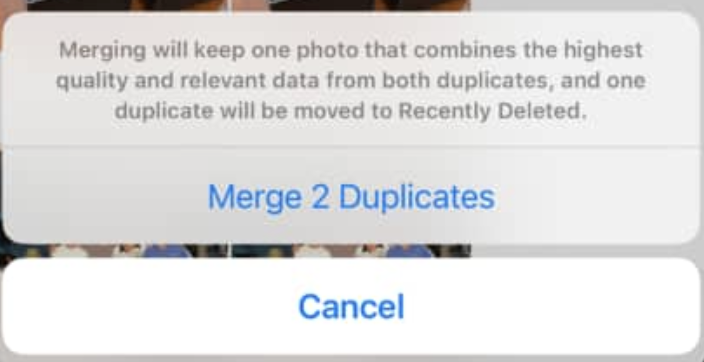
\includegraphics[width=0.4\textwidth]{images/duplicates.png}
\end{center}

\end{frame}

\begin{frame}
\frametitle{Column-Oriented?!}

Interestingly, we might want to use column-oriented storage in the warehouse rather than the standard row-oriented storage. 

There might be two advantages: 

(1) if we are fetching only a few attributes, we get exactly what we need rather than having to throw away parts of rows we don't need; 

(2) storing things of the same type makes compression possible. 

But the drawback is that accessing a single row means multiple I/O operations. 


\end{frame}

\begin{frame}
\frametitle{Mining}

With the data stored, now we want to use it.

 There are three kinds of information we could discover:

\begin{itemize}
	\item \textbf{Association Rules}
	\item \textbf{Sequential Patterns}
	\item \textbf{Classification Trees}
\end{itemize}

\end{frame}

\begin{frame}
\frametitle{Association}

We'll start off by looking at association. 

A credit score is a way of assessing the likelihood that a person borrowing money will repay the money.

The best way of predicting whether or not someone is likely to repay a loan is, of course, their previous behaviour. 

\begin{center}
	
\includegraphics[width=0.25\textwidth]{images/happening-again.jpg}
\end{center}

\end{frame}

\begin{frame}
\frametitle{Association}

But for someone who doesn't have a credit history, we might try to use some association data to predict: 

(1) whether we should lend this person money and 

(2) if so, at what interest rate.

\end{frame}

\begin{frame}
\frametitle{Association: Credit Scores}

Suppose there are four categories for credit: bad, average, good, and excellent. 

Then we need to figure out what are the key elements that determine someone's repayment history. 

We have some amount of data on an individual: place of birth, educational attainment, age, gender, income, marital status, and many more items. 


\end{frame}

\begin{frame}
\frametitle{Association: Credit Scores}

Some of the information we have is not relevant; some of it is. 

\begin{center}
	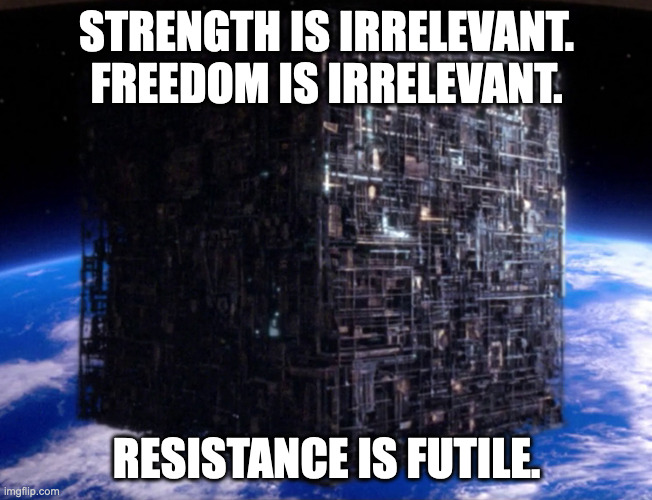
\includegraphics[width=0.4\textwidth]{images/futile.jpg}
\end{center}

What we are looking for is a statistical correlation that says, for example, repayment of a loan is correlated with higher income.


\end{frame}

\begin{frame}
\frametitle{Training Set}

The data that we have is our \alert{training set}. 

The training set is used to produce the rules by finding the correlations. 

What we should actually do is use a subset of the data as the training set. 

Then we verify the predictive power of the rules we have developed by looking at the rest of the data to see if the predictions match reality.


\end{frame}


\begin{frame}
\frametitle{Be Efficient}

Now, in theory we could use every piece of available data to make a prediction. 

We only care about those elements that have a correlation and predictive value. 

We might pick only a top few items, ranking them from strongest to weakest. 

Using those we can then build a tree that will be used to classify the creditworthiness of people for whom we have no (or limited) data.

\end{frame}

\begin{frame}
\frametitle{Seriously, Don't}

It's worth noting that sometimes data may point to certain correlations, but it would be unethical to use it. 

Discrimination based on elements like family origin, gender, religion, anything like that is unethical if not illegal in a given jurisdiction. 

\begin{center}
	
\includegraphics[width=0.4\textwidth]{images/disapproval-face.png}
\end{center}

We might have the data in our database, though, or be able to find it out.

It is still not okay to use.

\end{frame}


\begin{frame}
\frametitle{Credit Repayment}

Assume data we have says the biggest predictor of loan repayment is degree attainment; the next biggest is income. 


\begin{center}
\includegraphics[width=0.75\textwidth]{images/classification-tree}
\end{center}

\end{frame}


\begin{frame}
\frametitle{Educated Guessing}

It is important to note that these are predictions, guesses, really. 

Just because someone is predicted to have a good chance of repaying any loans made to them, does not actually mean that they will. 

We might say that good is a 75\% chance of on-time repayment. 

25\% of people who would be predicted to be in the ``good'' category would end up paying late at least once or defaulting (missing payments).

\end{frame}

\begin{frame}
\frametitle{Building Decision Trees}

Our plan is to choose a sequence of partitioning attributes. 

We use those to partition the data that we have so that we get ``pure'' leaves that contain only instances of a particular class. 

But there are good and bad ways to divide up the data. 

Suppose an insurance company wants to make some observations about who is at risk for car crashes. 

\end{frame}

\begin{frame}
\frametitle{Building Decision Trees: Auto Insurance}

Criteria under consideration might be the colour of the vehicle insured and the number of horsepower of the engine. 

At first glance your intuition might say that it is obvious that the colour of the car is not very important.

\begin{center}
	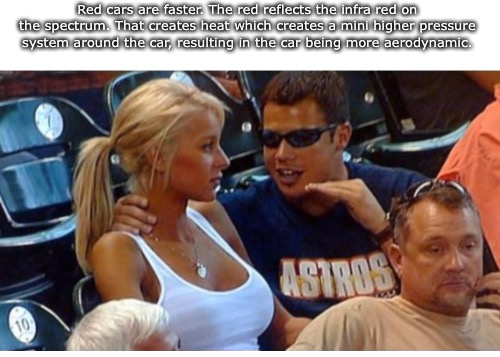
\includegraphics[width=0.4\textwidth]{images/redcar.png}
\end{center}

What we would like, however, is a way to quantify it.

\end{frame}

\begin{frame}
\frametitle{Building Decision Trees: Auto Insurance}

We can do so by treating this as an optimization problem: measure the purity of a data at the children nodes resulting by partitioning by that attribute. 

Choose the attribute that results in the highest purity.

\end{frame}

\begin{frame}
\frametitle{Gini Measure}

Suppose we have a set $S$ of training instances and there are $k$ classes. 

The fraction of instances in a class $i$ is $p_{i}$. 

Then we can calculate the Gini measure as:


$$\mbox{Gini($S$)} = 1 - \sum_{i-1}^{k}p_{i}^{2}$$

If all instances are in a single class, the Gini measure is 0.

Its maximum value is $1-1/k$ if every class is equal in size.

\end{frame}

\begin{frame}
\frametitle{Information Gain}

This can be used to calculate the information gain; how much we have learned. 

If $S$ is split into multiple sets, the purity of the split is calculated as:

$$\mbox{Purity($S_{1}, S_{2}, ... S_{n}$)} = \sum_{i = 1}^{n}\dfrac{|S_{i}|}{|S|} \mbox{purity($S_{i}$)}$$

Then information gain is calculated as purity($S$) $-$ purity($S_{1}, S_{2}, ... S_{n}$).

\end{frame}

\begin{frame}
\frametitle{Entropy}

Another measure is of entropy which is:

$$\mbox{Entropy($S$)} = - \sum_{i-1}^{k}p_{i} \log_{2} p_{i}$$

The entropy value is 0 if all instances are in a single class. 

It has a maximum value if all classes are equal in size.

\end{frame}

\begin{frame}
\frametitle{Information Content}

From that we can calculate information content as:

$$ - \sum_{i-1}^{n} \dfrac{|S_{i}|}{|S|}  \log_{2} \dfrac{|S_{i}|}{|S|} $$

And the best split for an attribute is then the one that gives the most benefit.

Information gain divided by information content.

\end{frame}

\begin{frame}
\frametitle{Bayesian Classifier}

Our choice of correlation criteria does not necessarily account for correlations between the criteria themselves. 

For example, degree attainment is correlated with higher income  in general and there may even be a causation relationship there.

It doesn't really matter (except to statisticians); all that we are concerned about is the correlation, the predictive power.


\end{frame}


\begin{frame}
\frametitle{Bayesian Classifier: Obligatory xkcd}

\begin{center}
	\includegraphics[width=0.7\textwidth]{images/correlation}
\end{center}


\end{frame}


\begin{frame}
\frametitle{Using Bayes Theorem}

Bayes' theorem: $P(A|B) = \dfrac{P(B|A)P(A)}{P(B)}$. 

Here's a quick example where only income is used as a predictor. 

Suppose that a person's income is \$76~000. 

This means they fall into the bucket for the range \$75~000 -- \$76~000.

\end{frame}


\begin{frame}
\frametitle{Using Bayes Theorem}

Looking at people who have a rating of excellent, the probability of income being in that range is 0.1. 

Looking at people who have a rating of good, the probability of income being in that range is 0.05.

 And if the overall fraction of people in excellent is 0.1 and the overall fraction in good is 0.3 we can plug and chug...
 
 \end{frame}


\begin{frame}
\frametitle{Using Bayes Theorem}
 
The probability of excellent for this person is .01 and for good it is 0.015. 

The highest probability is 0.015 so we go with that: this person is predicted to be in the category good, and that is the category they are assigned.

\end{frame}

\begin{frame}
\frametitle{Attributes Can Be Related}

The conditional probability of any particular attribute is highly dependant on the other attributes. 

In the worst case scenario, we would need to draw from a pool of people who are exactly alike on all relevant attributes to ensure that the prediction is good.

\end{frame}

\begin{frame}
\frametitle{Attributes Can Be Related}

So we will assume that all attributes have independent distributions: i.e., we can simply multiply them together. 

We know that isn't true, but it is sufficient for the job of estimation. 

\begin{center}
	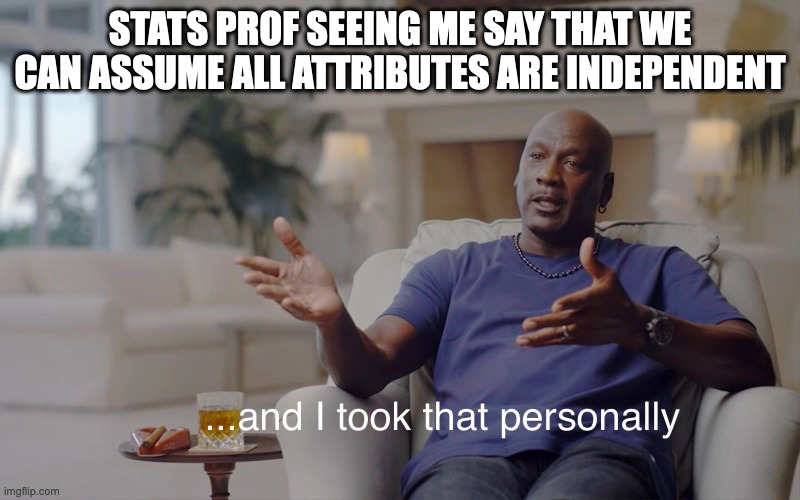
\includegraphics[width=0.5\textwidth]{images/personally.jpg}
\end{center}

\end{frame}

\begin{frame}
\frametitle{Association}

Remember that association is about events that are likely to take place at the same time; e.g., a customer who buys one item is likely to buy another. 

We are basically, once again, looking at statistics here. 

\end{frame}

\begin{frame}
\frametitle{Association}

If the user adds the Blu-Ray disk for ``Inception'' to their cart. 

To present a list of suggestions, we look at the history of purchases. 

What are the three items that appear in shopping carts most often alongside that film?

\end{frame}

\begin{frame}
\frametitle{Support and Confidence}

Rules for association have an associated \alert{support} as well as \alert{confidence}. 

Let's look at a quick shopping example. 

We have a simple corner store and it sells some basic supplies.

\end{frame}

\begin{frame}
\frametitle{Support}

Support is what fraction of the purchases satisfy the antecedent and the consequent. 

Remember that if the statement is P implies Q, the antecedent is P and the consequent is Q. 

So if the premise is that buying milk implies buying bread, milk is the antecedent and bread is the consequent. 

\end{frame}


\begin{frame}
\frametitle{Support}

If 0.001\% of all purchases include both milk and screwdrivers, then support for the proposition that milk implies screwdrivers is very low. 

If, however, 50\% of all purchases include both milk and bread, support for this rule is very high.

\end{frame}

\begin{frame}
\frametitle{Confidence}

Confidence is how often the consequent is true when the antecedent is true. 

The proposition of bread implies milk has a confidence of 80\% if 80\% of purchases of bread also include milk. 

A proposition with low confidence is probably not useful. 

\end{frame}

\begin{frame}
\frametitle{Confidence}

Keep in mind that P implies Q can have a different confident from Q implies P, even though they have the same support. 

That is to say, it might be the case that: \\
\quad 100\% of purchases for battery chargers include batteries.\\
\quad But only 10\% of purchases of batteries include battery chargers.


\end{frame}

\begin{frame}
\frametitle{What Do We Suggest?}

So: we want to find the items that are most likely to be purchased together. 

So first we find the sets of items that have large support (e.g., are likely to be purchased together). 

Then we look at the confidence level inside each set. Only those with sufficient confidence are offered up as suggestions. 

\end{frame}

\begin{frame}
\frametitle{Data Visualization}

To wrap up, a small digression about data visualization. 

A visualization helps users to look at large volumes of data and detect patterns. 

If data is presented well, then humans can see patterns in the data that might not otherwise be easy to detect. 
\end{frame}

\begin{frame}
\frametitle{Data Visualization}

\begin{center}
	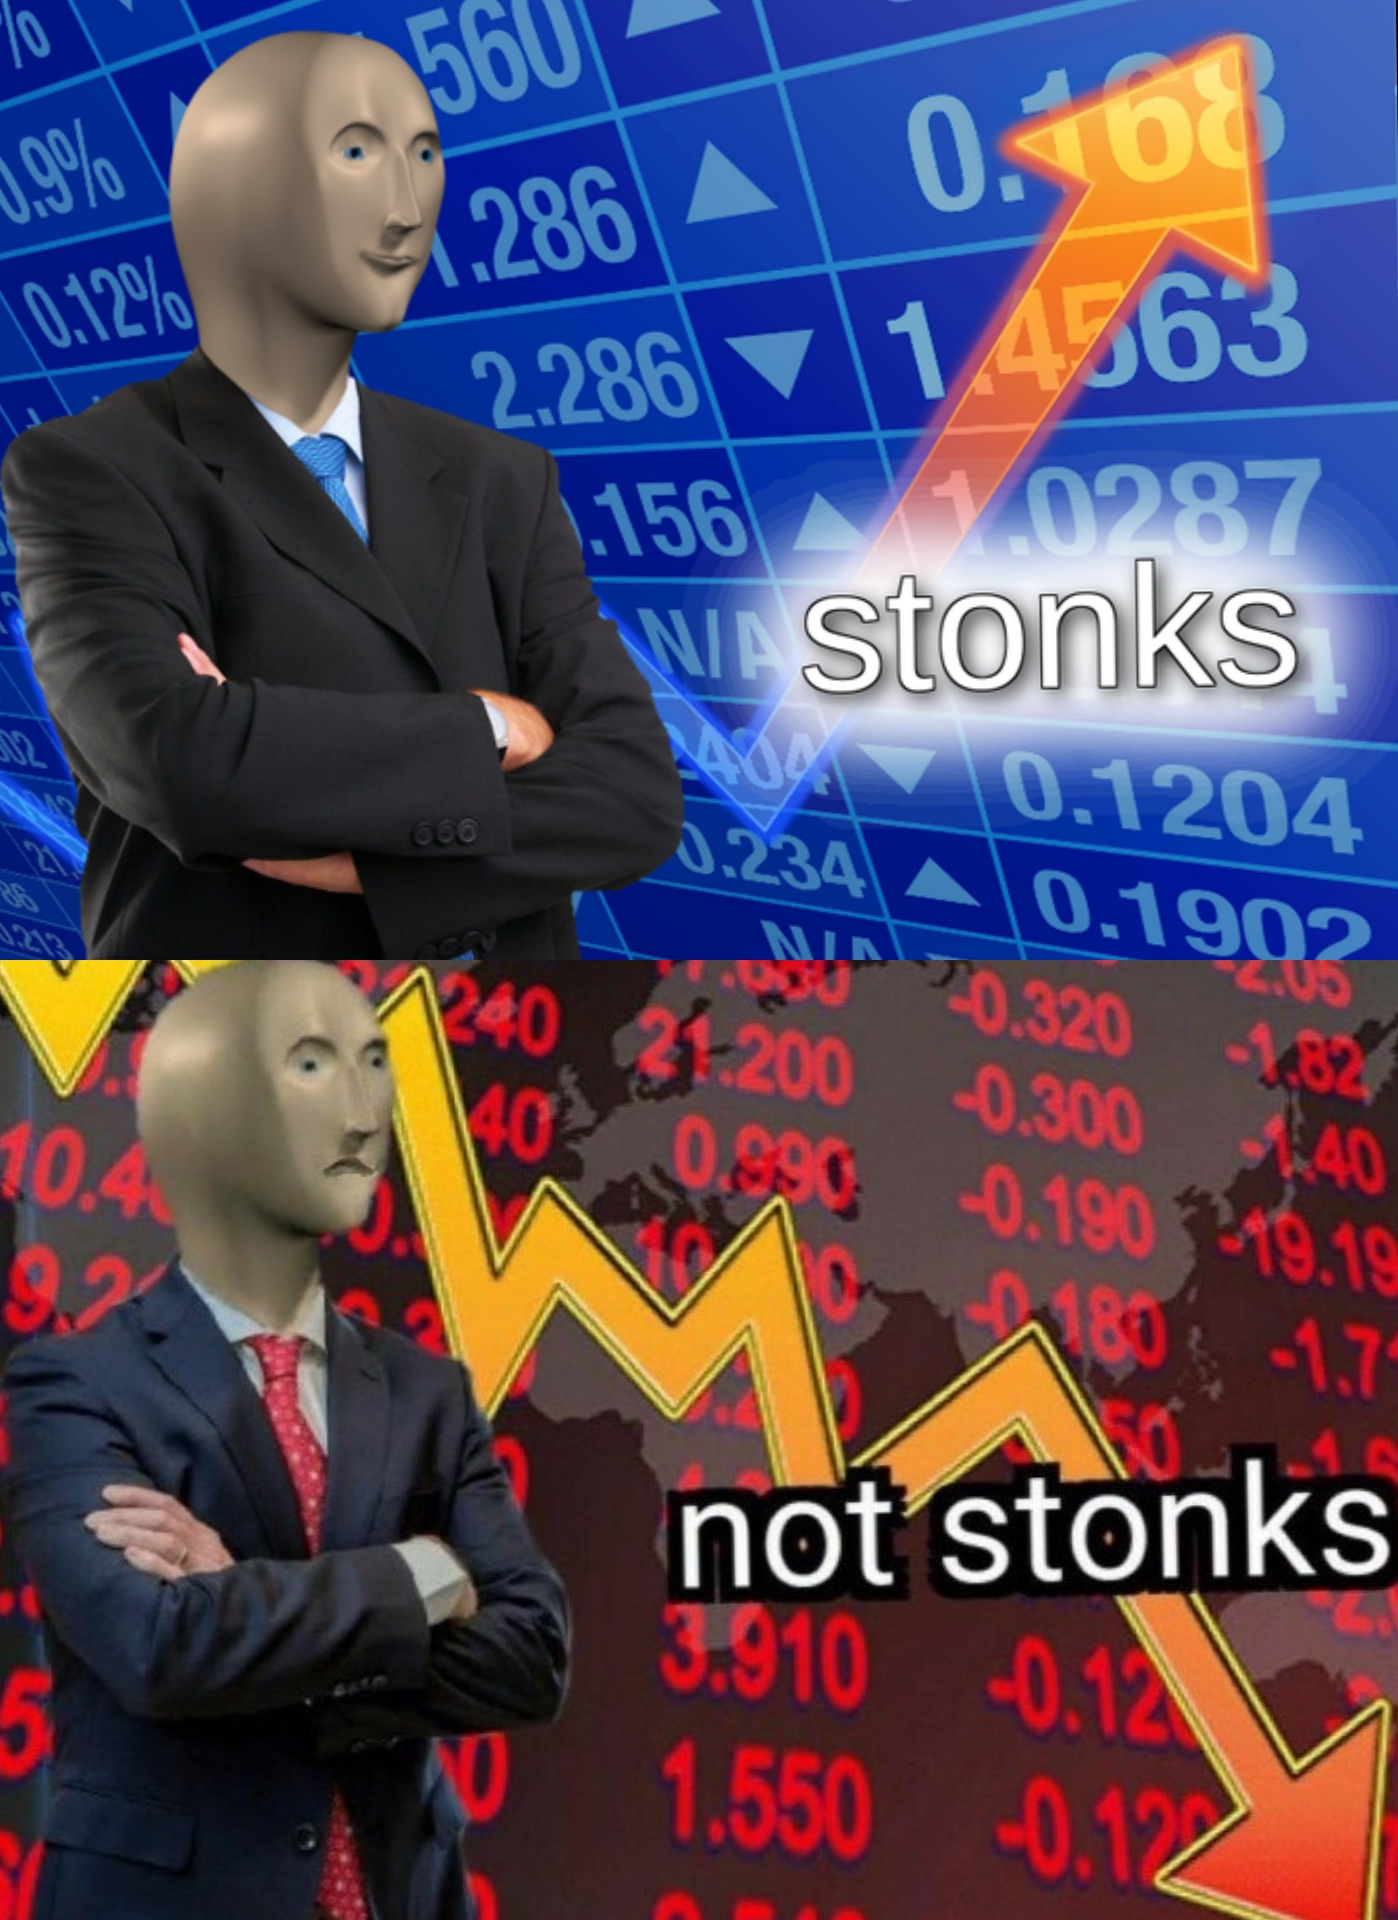
\includegraphics[width=0.4\textwidth]{images/stonks.jpg}
\end{center}

Bar charts, heat maps, line graphs can be effective ways of representing data.

\end{frame}




\end{document}

